% !TEX TS-program = pdflatex
% !TEX encoding = UTF-8 Unicode 
\documentclass[a4paper,11pt,openright,BCOR=15mm]{scrbook}

\usepackage[onehalfspacing]{setspace}    %   
\usepackage[utf8]{inputenc}
\usepackage[portuges,english]{babel}     
\usepackage[square,numbers]{natbib}
\usepackage{graphicx}               
\usepackage[pdftex]{hyperref}
\usepackage[T1]{fontenc}          
\usepackage{pdfpages}         
\usepackage{lettrine}    
\usepackage{booktabs}  
\usepackage{scrhack}   
\usepackage{scrlayer-scrpage}
\usepackage{ulem} % for underline
\usepackage{xcolor}
\definecolor{cinza1}{RGB}{200,200,200}
\definecolor{cinza2}{RGB}{70,70,70}
\usepackage{vhistory}	%% para versoes....
\newcommand\ChapterFont{}      % usar o tipo de letra normal
\newcommand\SectionFont{}
\pagestyle{scrheadings}
\ifoot[]{\raisebox{-32pt}{
\includegraphics[width=0.15\textwidth]{logos/logoisep}}}
\ofoot[]{\raisebox{-22pt}{
\includegraphics[width=0.10\textwidth]{logos/logo_DEI_big_transparente}}}
\cfoot[\pagemark]{\pagemark}
\automark[section]{chapter}
\usepackage{blindtext}   % \texto para demos 
\usepackage{listings}   %  para listagens com diferentes tipos de letra
\usepackage{fancyvrb}  %  para listagens de codigo 
\usepackage{float}
%%%%%%%%%%%%%%%%%%%%%%%%%%%%%%%%%%%%%%%%%%%%%%%%%%%%%%%%%%%%%%%%%%%%%%%%%%%%
\usepackage[mono=false]{libertine}
%%%%%%%%%%%%%%%%%%%%%%%%%%%%%%%%%%%%%%%%%%%%%%%%%%%%%%%%%%%%%%%%%%%%%%%%%%%%%%%%%%%%%%%%%
\begin{document}
	
	\selectlanguage{english}  
	\frontmatter
	
	\titlehead{
\includegraphics[scale=0.2]{figs/logoisep}
		\hfill 
\includegraphics[scale=0.115]{logos/logo_DEI_big_transparente}
	}  
	
	\title{Project (First Part) \\ \underline{Global report of group 200} 
		}
	\subtitle{QSOFT}
	
	\author{Master in Informatics Engineering - 2024/2025}        
	
	
\publishers
{
	1181180, \\1191526, \\1201100, \\1230210,\\1240485\\    \texttt{Version \vhCurrentVersion, \vhCurrentDate}\\
}         
  
	
	
	
	\date{Porto, \today} 
	
	
	\maketitle   
	
	\begin{versionhistory}
		\vhEntry{1}{2024-11-05}{Group 200}{Initial version}  
		\vhEntry{2}{2024-11-06}{Group 200}{Missing section in Report} 
		\vhEntry{3}{2024-11-07}{Group 200}{Final version} 
		
	\end{versionhistory}
	
	\cleardoublepage
	

	
	
	
	\tableofcontents
	\addcontentsline{toc}{chapter}{List of Figures}
	\listoffigures
	
	
	
	% \listoftables 
	
	\mainmatter 
	
	%% =================================
	
	
	%% =================================
	\chapter{Introduction}
	
	This document outlines the contributions made by Group 200 for the QSOFT course. The primary task was to examine and assess the quality aspects of an application named "Pet Clinic." The key aim was to evaluate whether the application aligns with the necessary quality standards and requirements for potential reuse in other projects. The report is organized into multiple sections, including Context, Task Allocation, Tools and Technologies, Standards, Goal-Question-Metric, and some Final Thoughts
	
	
	
	\chapter{Project under examination}
	
	The project was originally available at \url{https://github.com/spring-petclinic/spring-petclinic-rest.git}. This application allow user to manage a Pet Clinic, and have only few Aggregates with respective endpoints.
	
	Initially, each endpoint had specific authorization by "roles" and we chose to remove it in order to facilitate the entire work. (e.g.: Only admins could GET Pets)
	
		\section{Architecture}
		This project was implemented in Java, utilizing the Spring Boot. Its architecture follows a layered design approach, facilitating clear separation of responsibilities and enhancing the application’s scalability. Adopting a Domain-Driven Design (DDD) methodology, the system is divided into manageable domains, employing elements like entities, services, and repositories for accurate domain modeling and respects the Single Responsibility Principle.
		
		\begin{figure}[H]
			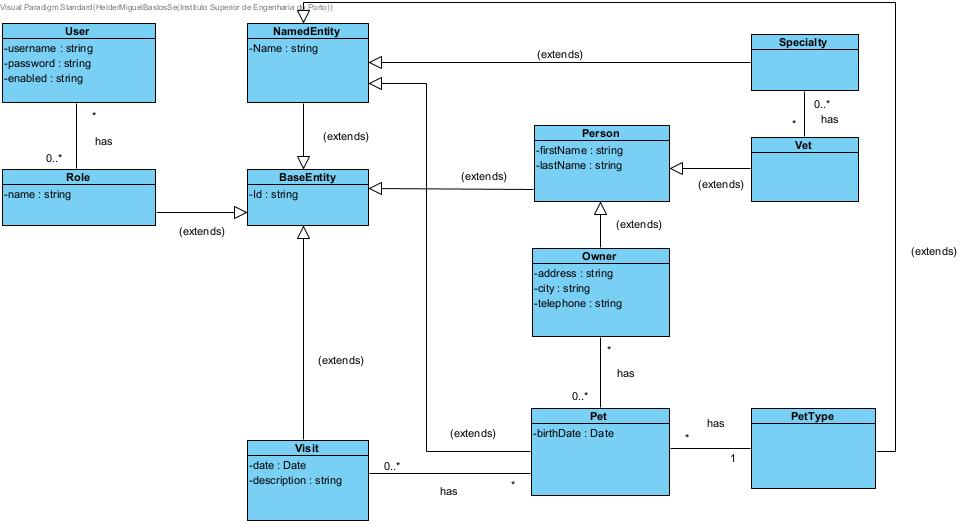
\includegraphics[width=\textwidth]{figs/MD.jpg}
			\caption{Domain Model Diagram}
			\label{fig:Domain Model Diagram}
			\centering
		\end{figure}
		
		Was we say before, the application architecture is divided in some layers:
		\begin{itemize}
			\item \textbf{Rest (Controller) Layer:} Handles HTTP requests and responses, directing them to the corresponding service for processing.
			
			\item \textbf{Domain Layer:} The domain layer represents the core business logic and rules of the application, encapsulating entities, value objects, and services that model real-world concepts and behaviors specific to the problem domain.
			
			\item \textbf{DTOs Layer:} They are simple objects used to transfer data between different parts of an application, often between the client and server or across layers, without exposing the internal details of the domain model.
			
			\item \textbf{Repository Layer:} The repository layer manages data access and persistence, providing a way to interact with the database by handling the retrieval, storage, and query of domain entities.
			
			\item \textbf{Mapper Layer:} The mapper layer is responsible for converting data between different layers of the application, typically transforming domain objects to data transfer objects (DTOs) and vice versa, ensuring smooth communication and data integrity across layers.
			
			\item \textbf{Service Layer:} The service layer contains the core application logic, coordinating operations between the repository and domain layers, and executing business processes to fulfill specific application requirements.
			
		\end{itemize}
		
		\section{Functionalities}\label{functionalities}

		This project serves as the backend of the Spring Pet Clinic, so it only provides the backend features. There are numerous functionalities for managing owners, veterinarians, and animals, which together complete a management of a pet clinic.

		For a brief resume, the main functionalities are :
		\begin{itemize}
			\item Owner
			\begin{itemize}
				\item Add, list, edit, and delete pet owners. 
				\item Get details of specific owner and his pets
			\end{itemize}
			\item Pet
			\begin{itemize}
				\item Add, list, edit, and delete pets associated with an owner. 
			\end{itemize}
			\item Vet
			\begin{itemize}
				\item Add, list, edit, and delete veterinarians. 
				\item Assign specialties for each Vet. 
			\end{itemize}
			\item Visit
			\begin{itemize}
				\item Add, list, and view pet visits. 
			\end{itemize}
		\end{itemize}
		
		\section{Conventions}
		The project follows a set of conventions to ensure consistency and readability in the project.
		Some of the detected conventions are:

		\begin{enumerate}
			\item Naming Conventions of Classes with Pascal Case (Figure \ref{pascalcase})
			\item Naming Conventions of Methods with Camel Case (Figure \ref{camelcase})
			\item Follows REST conventions using GET for reading, POST for creating, PUT for updating, and DELETE for deleting (Figure \ref{restConvention})
			\item Use of Annotations to define the behavior of the classes and data integrity (Figure \ref{annotationConvention})
		\end{enumerate}


		\begin{figure}[h!]
			\centering
			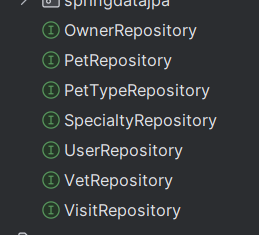
\includegraphics[width=0.5\linewidth]{figs/pascalCase.png}
			\caption{Class Names - Pascal Case}
			\label{pascalcase}
		\end{figure}

		\begin{figure}[h!]
			\centering
			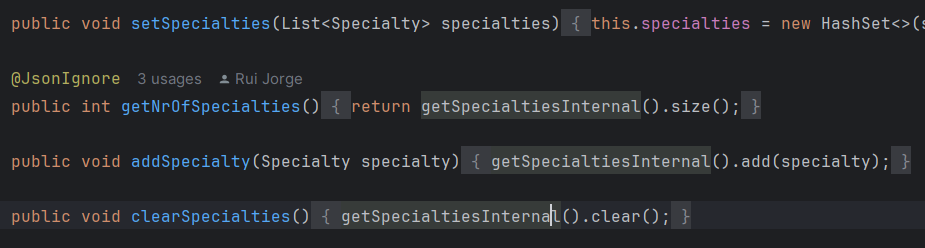
\includegraphics[width=0.5\linewidth]{figs/camelCase.png}
			\caption{Method Names - Camel Case}
			\label{camelcase}
		\end{figure}

		\begin{figure}[h!]
			\centering
			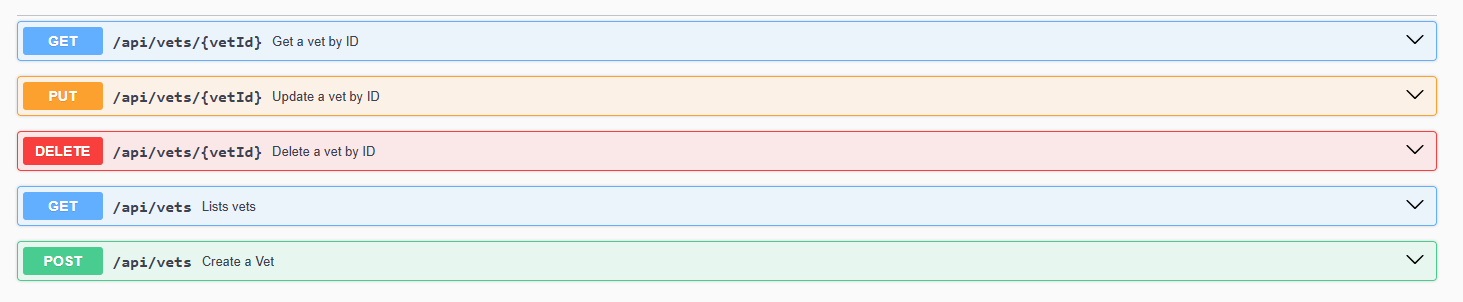
\includegraphics[width=0.5\linewidth]{figs/restConvention.png}
			\caption{REST Endpoints}
			\label{restConvention}
		\end{figure}
	
		\begin{figure}[h!]
			\centering
			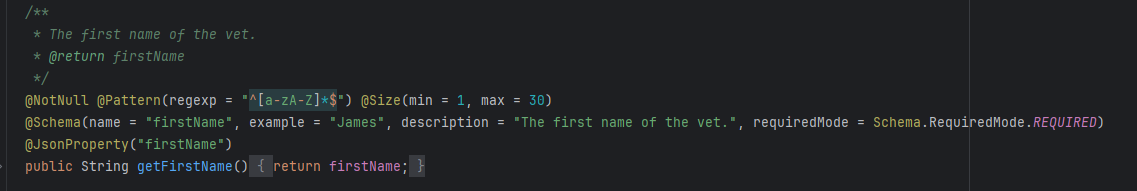
\includegraphics[width=0.5\linewidth]{figs/annotationConvention.png}
			\caption{Annotations of the Model Classes}
			\label{annotationConvention}
		\end{figure}

	
	%% =================================
	
	\chapter{Work distribution}
	This chapter describes the assignments of each student, as follows:\newline
		
		\begin{itemize}
			\item Student 1181180 - Owner Aggregate: 
			\begin{itemize}
				\item Functional correctness: JaCoCo Code Coverage on Owner Aggregate and full application
				\item Maintainability: Size and Complexity: Redudant Code and Number of Java Packages; Coupling and Structural Erosion: CCD - CCD Aggregate vs Application CCD; Instability and Cyclomatic complexity
				\item Maintainability of test code: JNose test Smells and some analyses
				\item Performance: JMeter and K6 Load, Soak and Stress test (POST + GET)
				\item Security: Input Validation, Dependency Vulnerabilities with Dependency Checker Plugin
				\item Architectural compliance: ArchUnit tests between packages and classes, inheritance, annotations, layers, and other architectural concerns
			\end{itemize}
			\item Student 1191526 - Vet Aggregate: 
			\begin{itemize}
				\item Functional correctness: JaCoCo Code Coverage on Vet Aggregate and full application
				\item Maintainability: Coupling and Structural Erosion: Maintainability Level; Size and Complexity:	Number of Types; Instability and Cyclomatic Complexity
				\item Maintainability of test code: JNose Test Smells
				\item Performance: JMeter and K6 Load, Stress and Soak test (PUT + GET)
				\item Security: Input Validation and Dependency Vulnerabilities with Dependency Checker Plugin
				\item Architectural compliance: ArchUnit tests focusing in Vet scope between packages and classes, inheritance, annotations, layers, and other architectural concerns
			\end{itemize}	
			\item Student 1201100 - Specialty Aggregate: 
			\begin{itemize}
				\item Functional correctness: JaCoCo Code Coverage on Specialty Aggregate and full application
				\item Maintainability: Coupling and Structural Erosion: Normalized Cumulative Component Dependency; Size and Complexity: Number of Statements and Number of Statements in Fully Analysed Code;
				\item Performance: JMeter and K6 Load, Soak and Stress test (GET + POST)
				\item Security: Input Validation and Dependency Vulnerabilities with Dependency Checker Plugin
				\item Architectural compliance: ArchUnit tests focusing in Specialty scope between packages and classes, inheritance, annotations and layers
			\end{itemize}
			\item Student 1240485 - PetType:
			\begin{itemize}
				\item Functional correctness: Jacoco Code Coverage on PetType Aggregate and full application
				\item Maintainability: Coupling and Structural Erosion: ACD; Size and Complexity Metric: Number of Components or Source Files
				\item Maintainability of test code: JNose Test Smells report and analysis
				\item Performance: JMeter and K6 Load/Soak/Stress tests (GET and POST)
				\item Security: Input Validation, Dependency Vulnerabilities with Dependency Checker Plugin
				\item Architectural compliance: ArchUnit tests focusing in PetType scope between packages and classes, inheritance, annotations, layers and other architectural concerns
			\end{itemize}	
			\item Student 1230210 - Pet:
			\begin{itemize}
				\item Functional correctness: Jacoco Code Coverage on Pet Aggregate and full application
				\item Maintainability: Coupling and Structural Erosion: Propagation Cost; Size and Complexity Metric: Total Lines and Code Comment Lines
				\item Maintainability of test code: JNose Test Smells report and analysis
				\item Performance: JMeter Load/Soak/Stress tests (GET and POST)
				\item Security: Input Validation, Dependency Vulnerabilities with Dependency Checker Plugin
				\item Architectural compliance: ArchUnit tests focusing in Pet scope between packages and annotations and other architectural concerns
			\end{itemize}
		\end{itemize}
		

	
	
	%% =================================
	
	\chapter{Technologies }
	 \section{JMeter}
	 Apache JMeter is an open-source software tool designed for testing and measuring the performance of applications, especially web applications and APIs. Originally created to test web applications, it has since expanded to handle a variety of applications, servers, and protocols, making it a popular choice for load and performance testing.
	
	\begin{itemize}
		\item Load Testing: JMeter allows you to simulate heavy loads on a server, group of servers, network, or object, to test its strength and analyze overall performance.
		\item Performance Testing: It provides insights into system performance under different scenarios, like simultaneous users or requests, response times, and failure rates.
		\item API Testing: JMeter is frequently used to test APIs. It can simulate requests, validate responses, and track performance over time.
		\item Protocol Support: JMeter supports multiple protocols, such as HTTP, HTTPS, FTP, SOAP, REST, TCP, and others.
		GUI and CLI Modes: JMeter has a graphical user interface (GUI) for designing and running tests and a command-line mode (CLI) for running tests in headless environments, often used in CI/CD pipelines.
		\item Extensibility: JMeter supports plugins, allowing users to extend its functionalities with additional samplers, listeners, and functions.
	\end{itemize}	
	
	\section{K6}
	K6 is an open-source tool for performance testing web applications and APIs, allowing developers to write test scripts in JavaScript. It is designed for load and stress testing, supporting thousands of virtual users and providing detailed metrics like response time, throughput, and error rates. Ideal for CI/CD pipelines, k6 integrates with monitoring tools like Grafana, making it a popular choice for identifying bottlenecks and ensuring application scalability.
	
	\section{ArchUnit}
	ArchUnit is a Java library designed to test and enforce architectural rules in codebases. It allows developers to define and validate architectural constraints within their Java projects using unit tests. ArchUnit helps teams ensure that their code follows certain structural guidelines and design principles, such as enforcing layering, module boundaries, and package dependencies.
	
	With ArchUnit, you can write tests that assert whether your code adheres to specific architectural patterns, like ensuring that certain classes reside in particular packages or that no direct dependencies exist between certain layers of your application. The rules you define can range from simple package dependency checks to more complex architectural validations involving class relationships, annotations, and inheritance structures.
	
	\section{SonarGraph}
	Sonargraph is a software analysis and quality management tool designed to help developers and teams monitor and improve the structure, quality, and maintainability of their codebase. It performs static code analysis to identify common issues such as code smells, architectural violations, and dependency problems, making it easier to manage the complexity of large projects. Sonargraph also allows teams to define and enforce architectural rules, helping maintain a clean and consistent design throughout the project. It provides insights into dependency management, highlighting unwanted coupling between components, and visualizes the relationships between classes, packages, and modules.
	
	By computing various metrics, such as cyclomatic complexity, coupling, and cohesion, Sonargraph helps teams quantitatively assess code quality. It also identifies code duplication, which can simplify maintenance and reduce redundancy. The tool’s interactive visualization features make it easy for teams to explore and understand complex codebases, while its integration with continuous integration systems ensures that quality checks are part of the development process. Sonargraph is particularly useful for identifying architectural issues, guiding refactoring efforts, and maintaining high code quality over time, especially in large or evolving codebases.
	
	\section{Dependency Check plugin}
	The Dependency Check plugin helps you find security problems in the libraries your project uses. It checks if any of the libraries have known security issues by comparing them to a security database. If it finds a problem, it tells you what the issue is and how to fix it.
	
	The plugin works with tools like Maven, Gradle, or Jenkins, and can automatically check your project every time you build it. This helps you catch security issues early and keep your project safe. You can also set it to stop the build if it finds a serious problem, making sure you don’t add security risks to your code.
	
	\section{JNose}
	Jnose is a tool that helps find security problems in Java projects that use native code. It checks for issues in how Java and native code interact, like unsafe actions or memory problems. It helps make sure that using native code in a project doesn’t introduce security risks.
	
	\section{Java Code Coverage (JaCoCo)}
	JaCoCo is an open-source toolkit designed for measuring code coverage within a project and generating detailed visual reports. It tracks line and branch coverage based on the code exercised by unit tests, providing insights through highlighted lines of executed code and showing the total percentage of code coverage for each method.
	
	%% =================================
	\chapter{Conventions }
	The group used GitHub Issues in order to associated each commit with a issue. The following figure show the Issues used:
	\begin{figure}[H]
		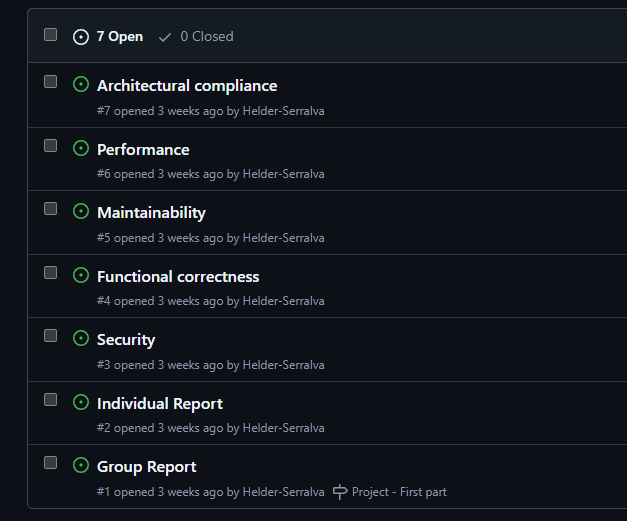
\includegraphics[width=\textwidth]{figs/Issues.png}
		\caption{GitHub Issues}
		\label{fig:Issues}
		\centering
	\end{figure}
	
	\chapter{Goal Question Metric Approach}
	\section{Plan}
	
	The figure below represent the group GQM Diagram. It was made in an initial phase with a lack of knowledge of Metrics. Also that, most of then, represented below are used by different members of group but some are used a lot.
	
	Despite all this, with the initial diagram we are able to say whether the application meets all the requirements raised, as we will see later.
	
	\begin{figure}[H]
		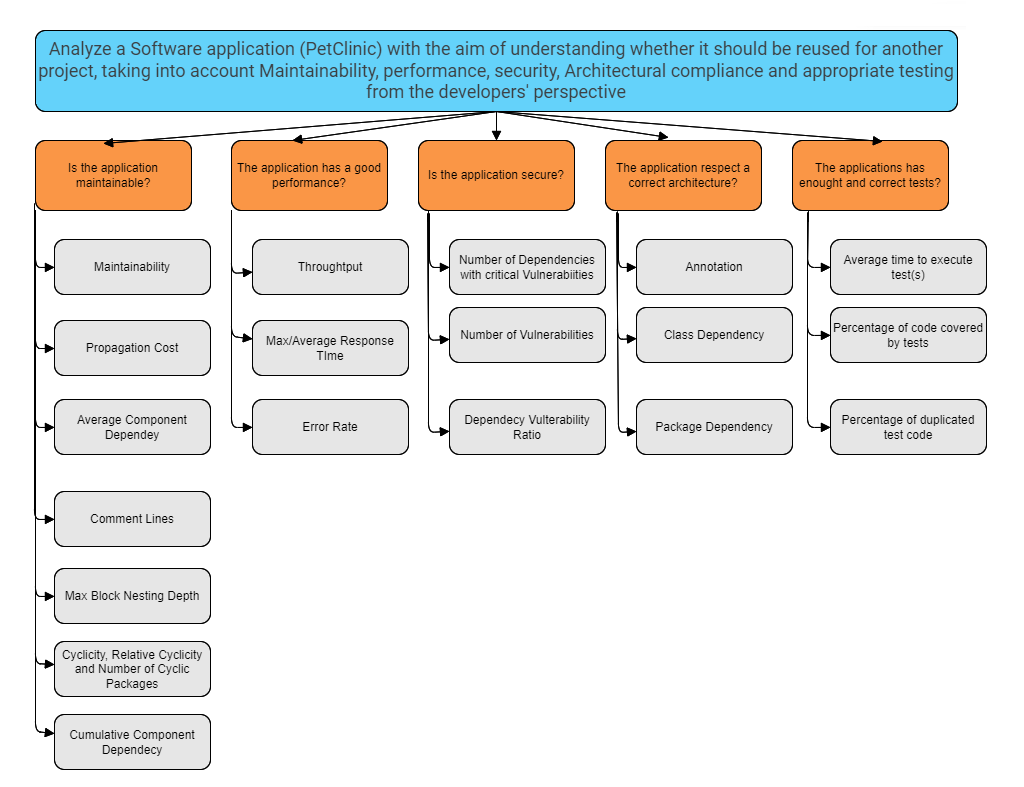
\includegraphics[width=\textwidth]{figs/GQM.png}
		\caption{GQM Diagram}
		\label{fig:GQM}
		\centering
	\end{figure}
	
	
	\section{Answering questions}
	Each group member focused on a different aggregate, with all member also assigned to review the application as a whole. The analysis and responses presented here are based on some specific aggregates: owners, vet and pet. To determine if the application fulfills its intended purpose, we’ll now address the GQM (Goal-Question-Metric approach).
	
	In order to rank each Question of GQM, we defined a scale from 0\% to 100\%.
	
			\subsection{Is the application maintainable?}			
				The project scores well on maintainability, especially considering its size and complexity, but falls short on cyclical dependencies have been identified, impacting overall structure.			
				Also that, the project has a shortage amount of tests without comments and the Controller layer's is the only one with sufficient tests.		
				Despite this, the group evaluates it with a score of 75\%.
			
			\subsection{The application maintainable has good performance?}			
				Regarding performance, it depends on several factors and it is difficult to reach a conclusion. There were members of the group managing to test with a thousand users and without returning an error, others with two hundred users already had requests with errors.			
				What was common to everyone was the success of the Load tests, in normal environments. However, we would have liked to have simulated more user fluctuations.			
				However, taking a group average we obtain a value of 80\%.
			
			\subsection{Is the application secure?}			
				Although the application has few dependencies on packages, some of them have vulnerabilities, most of which simply require updating and subsequent testing.		
				In terms of input validations, some are present, more than we expected, but they can still be improved.			
				Despite not being mentioned in any metrics, the fact that the API does not have authentication and 	authorization was withdrawn is a serious security flaw.		
				The group gives a score of 75\%.
			
			\subsection{The application respect a correct architecture?}		
				The application mostly respects the implemented architecture (layered architecture), therefore the value to be given at this point is 90\%, with the main failure being the Cycle test.
			
			\subsection{The application has enough and correct tests?}
				The application could have a few more tests so that all branches were tested, but in the main packages, the coverage ends up being above the median value, which indicates something positive but not perfect. Some improvements in terms of testing conditions in methods could be made to improve this topic.
				The lack of Lazy Tests and Tests Smells is also a positive point.
				The group gives a score of 60\%.
			
	\section{Analysing goal}

	If we were to take an average from the previous chapter, it would give a result of around 75\%, which is consistent with what each element did in their individual work.
	As such, in our opinion, the application could be used in any other context with small tasks. These details do not compromise the API at any level, however they are issues that can easily be reviewed and improved.
	
	\chapter{Conclusion}

	This work was very important for us to define Quality principles in an application (web) and learn several metrics and tools that we were unaware of many of them.
	However, it was a job that required a lot of time, making its completion more difficult. However, all requirements were apparently met and documented.


	
	\bibliographystyle{ACM-Reference-Format}
	\renewcommand\bibname{References}
	\bibliography{ref}
	\label{references}
	\addcontentsline{toc}{chapter}{References}
	
\end{document}